\chapter{Taking Action}

\section{Teams}
Now, check the Math Club Teams and see if anything needs updating or changing.
This is the base grounds for all information so make sure that 
that resources, links, competitions are all up to date.

\section{Creating PPTs}
You may use past year's ppt as inspiration. \\\\ Here is the general structure:

\begin{enumerate}
    \item Intro Page
    \item When + Where [Friday, Dr. Lu N-272] 
    \item Competitions  
    \item Tutoring \& Volunteer Hours 
    \item Final Take Aways: 
            \begin{itemize}
                \item Fridays N-272  | Can Drop out 
                \item  \# Competitions through the Year 
                \item  Tutoring Volunteer Hours 
                \item  Math Wizard/ academic weapon    
            \end{itemize}
    \item Form [Questions \& Attendance] 
            \begin{itemize}
                \item Name, Email, Grade
                \item AMC 10/12 
                \item Purpose for joining
            \end{itemize}

\end{enumerate}

\section{Club Meeting Plans}
This is where you decide what will happen during club meetings.

\noindent
Here is the general structure:
    \begin{enumerate}
        \item Set-Up Math Club [HDMI + Activities]
        \item Wait for people to come 
        \item Start [bang the gong if you want]
        \item Split into Activities
        \item End + Thanks
        \item REPEAT 29x~ Meetings
    \end{enumerate}

\section{Club Fair Prep}
During the 2nd or 3rd week of September, there will be a club fair for all of the clubs.
This is Math Club's first impression to any outsiders and this is our steady source of new members.
\newline
\newline
Some interesting topics this are:

\begin{itemize}
    \item Math Problem Activity
    \item Become a Math Wizard 
    \item Awards/Medals
    \begin{figure}[H]
        \centering
        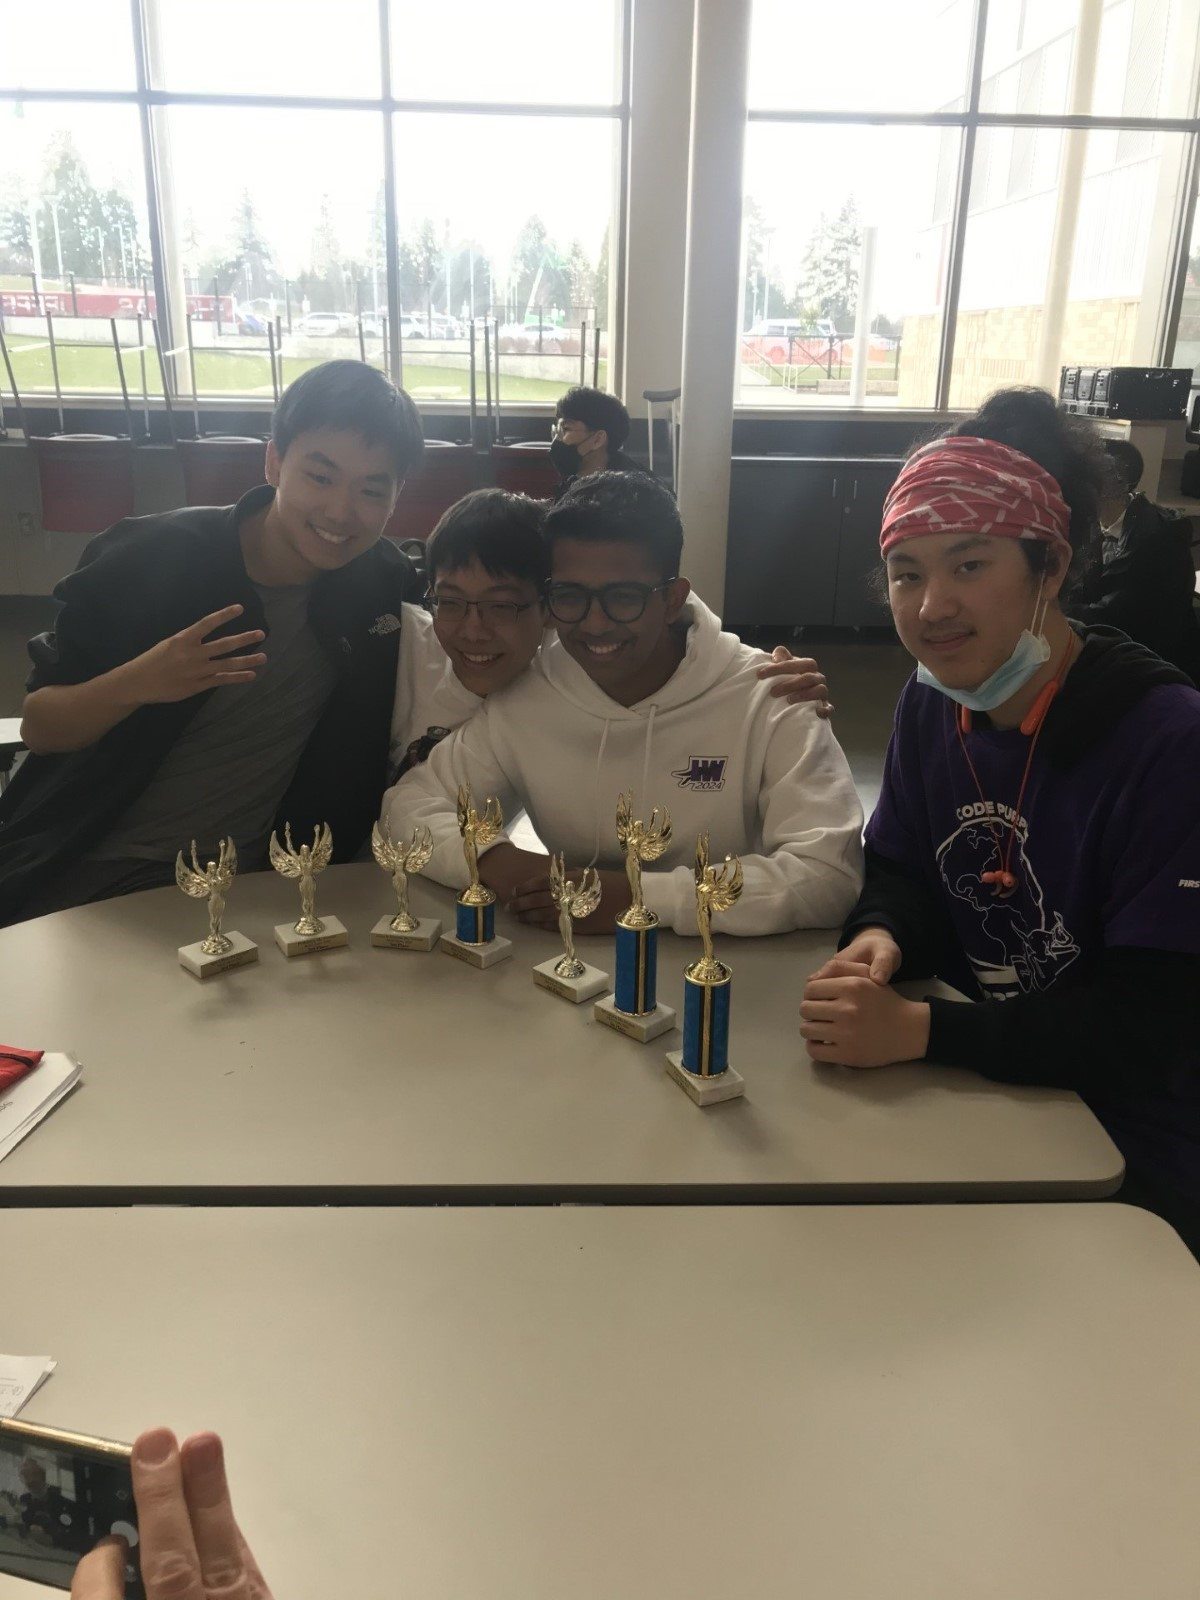
\includegraphics[width=.5\textwidth,height=.5\textheight,keepaspectratio]{example.png}
        \caption{2022-2023 MAO Spring Classic Competition: Logan Chu, Brice Liu, Amish Patra, Bryan H [Left to Right]}
        \label{fig:old competition image example}
    \end{figure}
\end{itemize}

\section{Fundraising}
After everything, now to acquire funds.
First know which businesses students usually go to and compile a hit-list.
Go to the businesses and ask the manager if they are able to make a fundraising deal.

If that doesen't go well, apply for an ASB Grant by contacting one of the ASB leadership members.
Then, volunteer at concessions for funding also.

\section{Officer Positions}
This wayyyy later on near June. If you have \key{completely finished} the above,
read in the \hyperref[sec:Officer]{ Endgame section} on this. 